%% 2.2 Elaborazione dati e risutati quantitativi
In questo paragrafo si riportano i dati elaborati, il calcolo delle misure indirette e la valutazione degli errori.\\
Per le grandezze per le quali si sono fatte più misure (tranne per il tempo) si è considerata come stima migliore la media, mentre come incertezza la semidispersione delle misure.\\
Nel caso in cui alcune incertezze valutate con la semidispersione siano risultati non sensati rispetto al setup sperimentale (per esempio incertezze troppo basse), allora si è andati a considerare la risoluzione dello strumento come incertezza.

\subsubsection*{Metodo geometrico}
I valori dei diametri $d_i$ sono:
    \begin{align*}
        d_1 &= (7.86 \pm 0.09) \textrm{ mm} \\
        d_2 &= (15.94 \pm 0.01) \textrm{ mm} \\
        d_3 &= (57.98 \pm 0.01) \textrm{ mm} \\
        d_4 &= (99.88 \pm 0.01) \textrm{ mm} \\
        d_5 &= (120.04 \pm 0.01) \textrm{ mm} 
    \end{align*}
Per le profondità $p_i$ e lo spessore del toroide più esterno $z_4$ si riportano i seguenti valori:
    \begin{align*}
        p_1 &= (8.1 \pm 0.1) \textrm{ mm} \\
        p_2 &= (3.09 \pm 0.05) \textrm{ mm} \\
        p_3 &= (13.14 \pm 0.05) \textrm{ mm} \\
        z_4 &= (29.96 \pm 0.01) \textrm{ mm} \\
    \end{align*}
Attraverso un'analisi geometrica della sezione assiale del disco, riportato in Fig. \ref{profondità} a pag. \pageref{profondità}, i spessori dei primi tre toroidi sono risultati:
    \begin{align*}
        z_1 &= (26.1 \pm 0.4) \textrm{ mm} \\
        z_2 &= (9.9 \pm 0.2) \textrm{ mm} \\
        z_3 &= (3.7 \pm 0.1) \textrm{ mm}
    \end{align*}
in cui gli errori sono stati calcolati secondo la propagazione degli errori considerando l'incertezza massima.\\

Per il calcolo del momento d'inerzia, ricorrendo alla formula (\ref{I_G}) a pag. \pageref{I_G}, si è ottenuto il valore di 
$$I_G = 4.91 \cdot 10^{-4} \textrm{ kg} \cdot \textrm{m}^2$$
Per la valutazione dell'errore si è ricorso al metodo della propagazione dell'errore con derivate, procedimento mostrato a App. \ref{errore_I_G} a pag. \pageref{errore_I_G}.\\
Dunque il valore finale di $I_G$ è di
$$I_G = (4.91 \pm 0.08) \cdot 10^{-4} \textrm{ kg} \cdot \textrm{m}^2$$

\subsubsection*{Metodo dinamico}
Per il metodo dinamico il valore della massa del disco era già stato fornito \textit{a priori}: 
$$m = (226.0 \pm 0.5) \textrm{ g}$$
Le misure dell'altezza di caduta, del diametro del perno e del filo sono stati:
\begin{align*}
    h_o &= (35.5 \pm 0.1) \textrm{ cm} \\
    d_p &= (0.42 \pm 0.03) \textrm{ mm} \\
    d_f &= (3.01 \pm 0.01) \textrm{ mm}
\end{align*}
Le misure del tempo di caduta del disco sono state raccolte in bin da 0.1 s, con occorrenze per ogni bin indicato nella Tab. \ref{tab_tempi_di_caduta_2}.
\begin{table}[htp]
    \begin{center}
        \begin{tabular}{||c|c||}
            \hline
            \hline
            \multicolumn{2}{||c||}{Tempi di caduta}\\
            \hline \hline
            tempo [s] & occorrenze \\
            \hline
            7.2 & 1\\
            7.3 & 7\\
            7.4 & 18\\
            7.5 & 9\\
            7.6 & 4\\
            7.7 & 1\\
            \hline
            \hline
        \end{tabular}
    \end{center}
    \caption[\small Tabella di tempi di caduta - occorrenze.]{\small Sono indicati i numeri di occorrenze dei tempi di caduta del disco per bin ampi 0.1 s. Si nota che il valore del tempo di caduta medio è di 7.43 s.}
    \label{tab_tempi_di_caduta_2}
\end{table}\\
Analizzando graficamente i dati della Tab. \ref{tab_tempi_di_caduta_2} si hanno ottenuto due grafici d'istogramma: il primo indica il numero delle occorrenze per bin (Fig. \ref{istogramma_tempi_di_caduta}), il secondo invece indica la frequenza dei valori in ogni bin (Fig. \ref{distribuzione_tempi_di_caduta}).
     \begin{figure}[htbp]
        \centering
        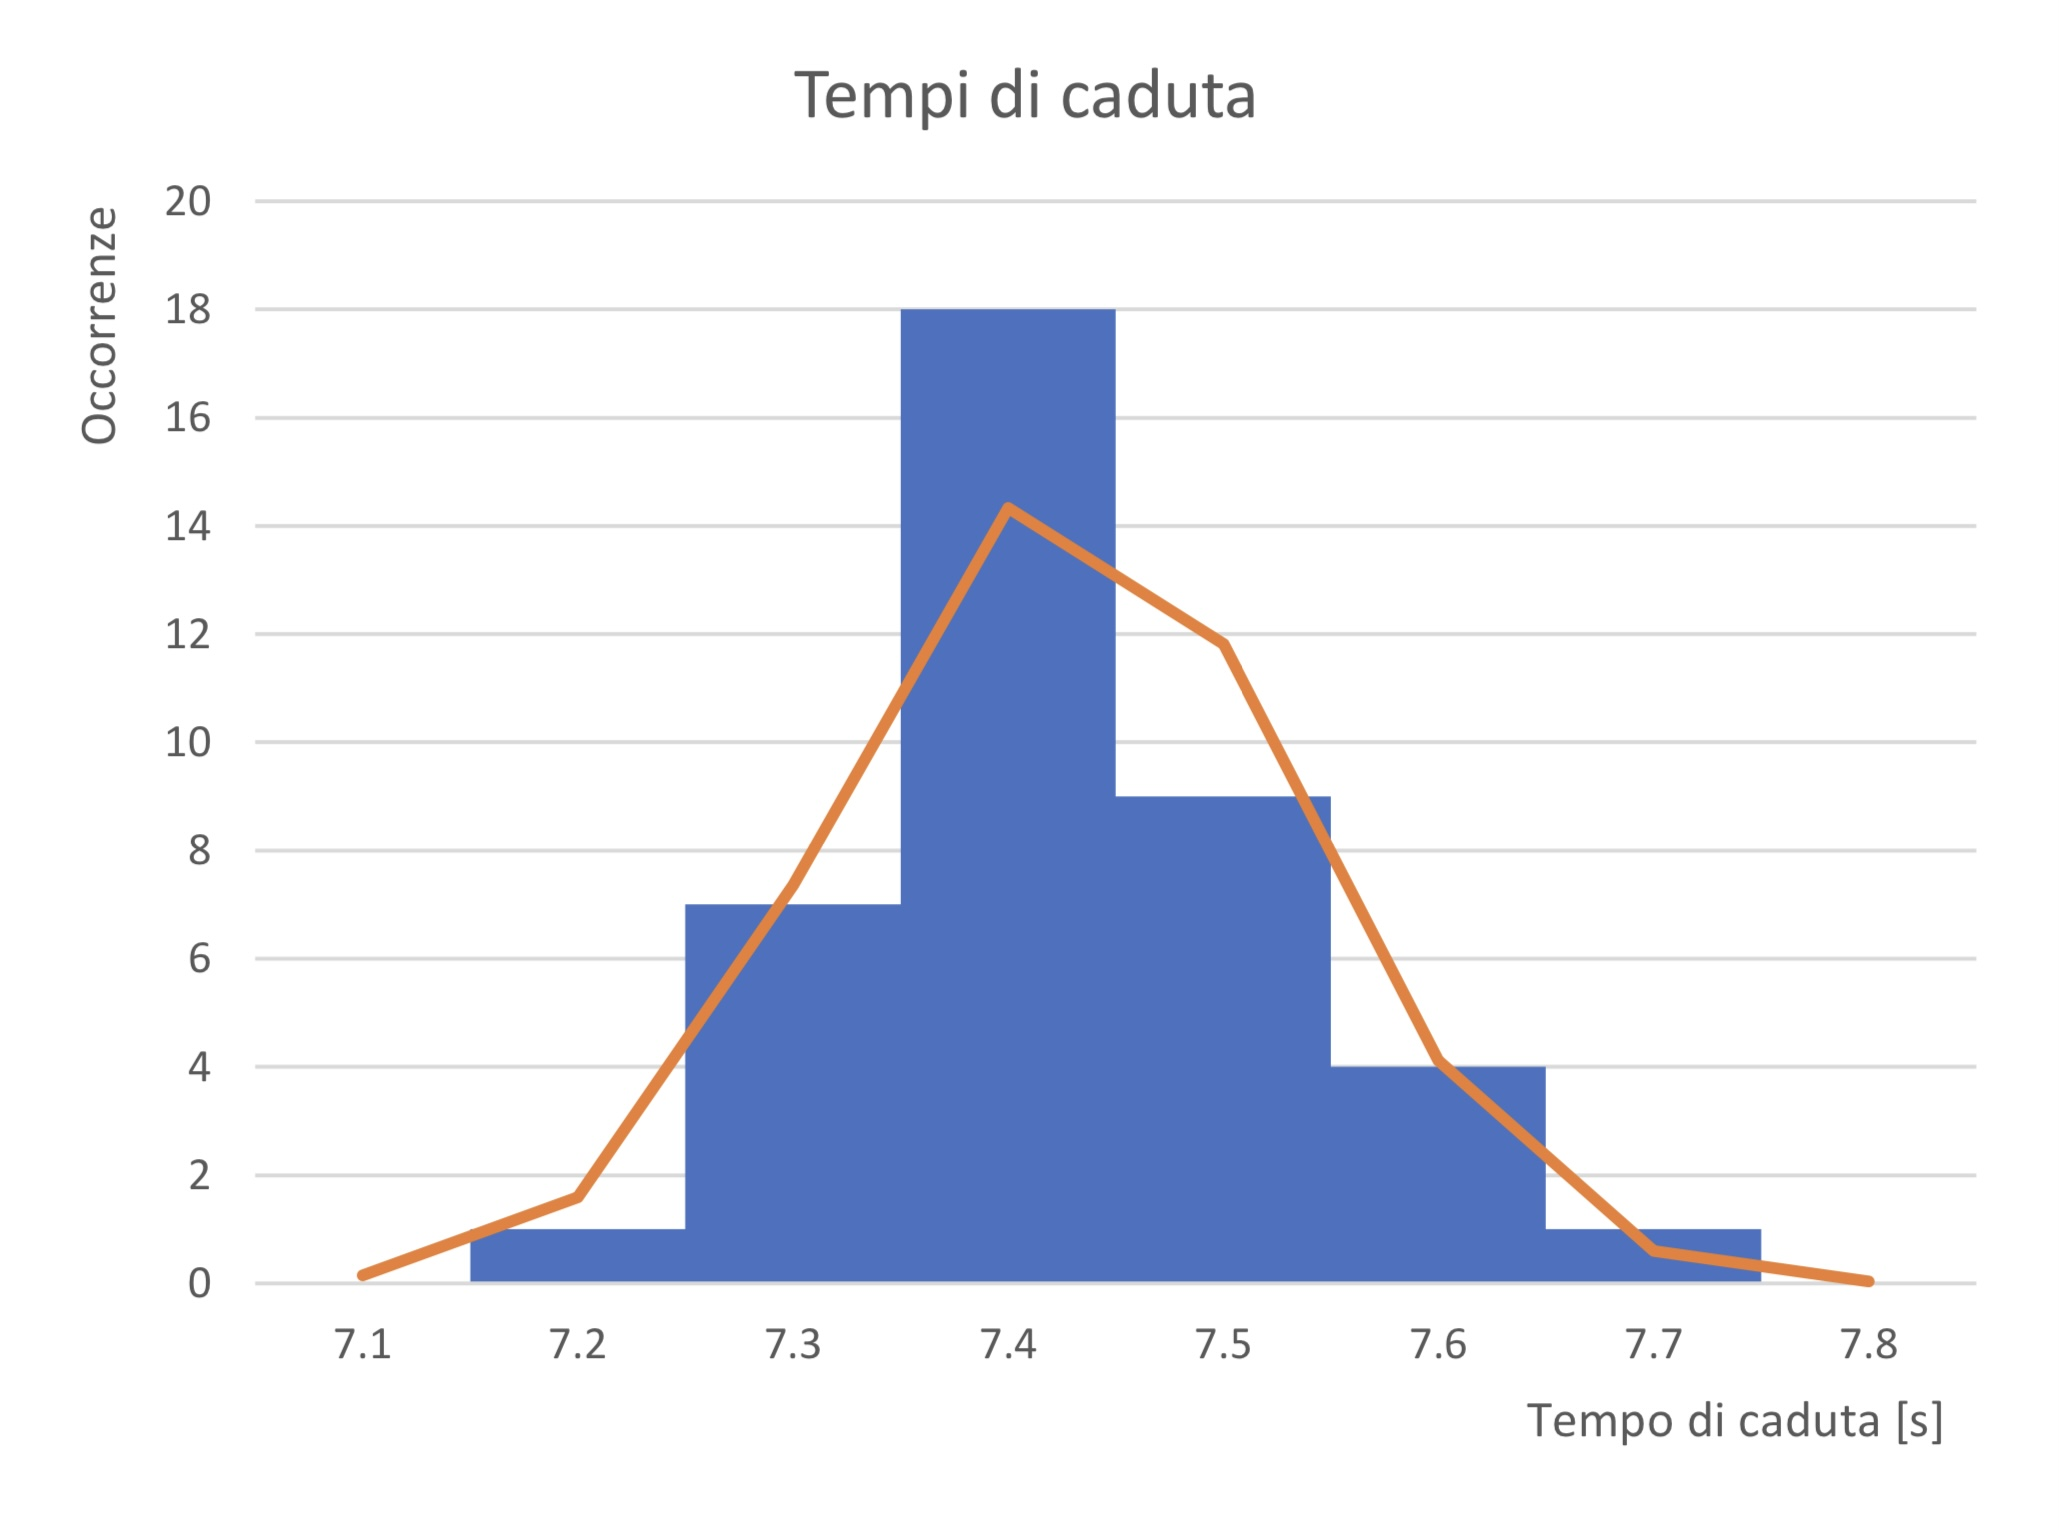
\includegraphics[width=\textwidth]{image/Istogramma_tempi_di_caduta.jpeg}
        \caption[\small L'istogramma del conteggio dei tempi di caduta del disco.]{\small Nell'istogramma sono riportati il numero di occorrenze (sull'asse delle ordinate) in corrispondenza di ogni bin da 0.1 s (sull'asse delle ascisse). Invece la linea spezzata arancione rappresenterebbe il valore atteso secondo la gaussiana con media e deviazione standard calcolato con i dati riportati in Tab. \ref{tab_tempi_di_caduta_2}.}
        \label{istogramma_tempi_di_caduta}
    \end{figure}
    
    \begin{figure}[htbp]
        \centering
        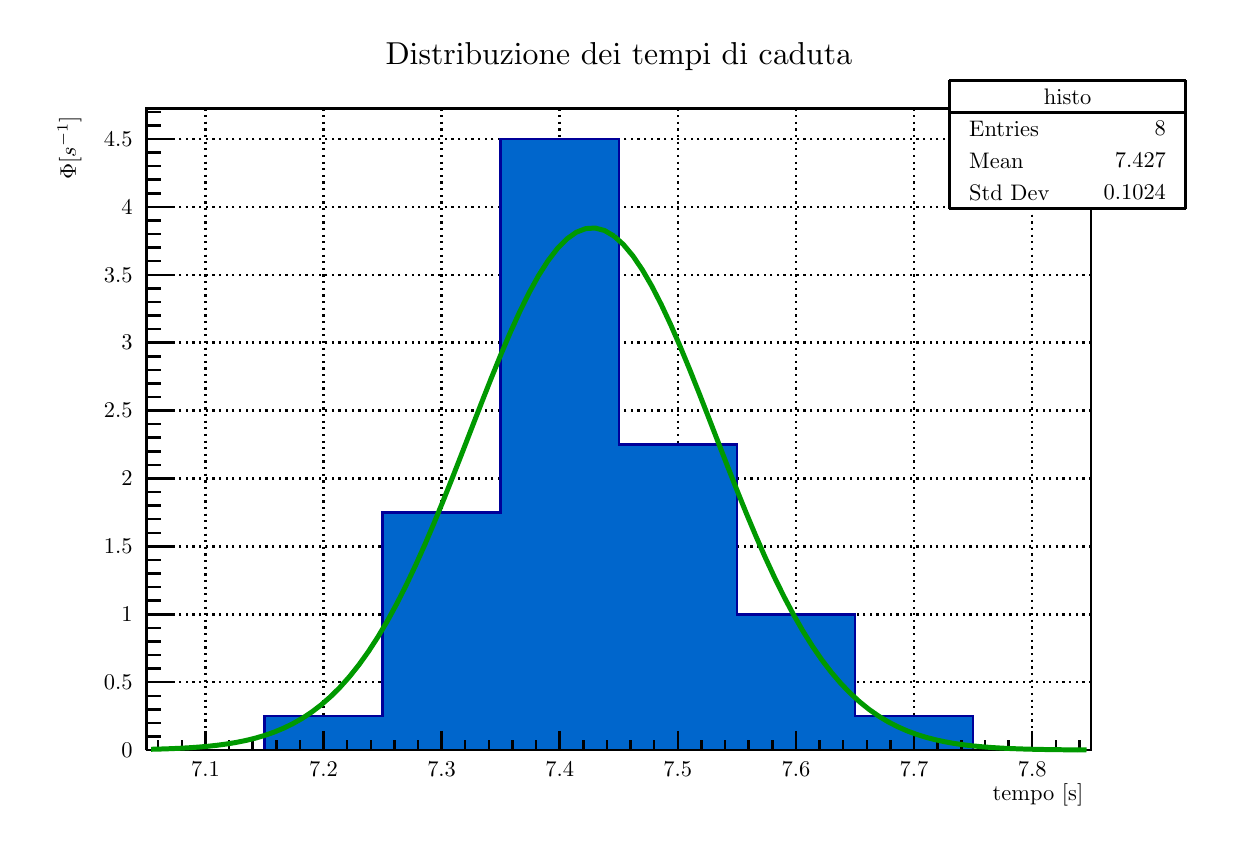
\begin{tikzpicture}[scale = 0.75, every node/.style={scale=0.75}]
\pgfdeclareplotmark{cross} {
\pgfpathmoveto{\pgfpoint{-0.3\pgfplotmarksize}{\pgfplotmarksize}}
\pgfpathlineto{\pgfpoint{+0.3\pgfplotmarksize}{\pgfplotmarksize}}
\pgfpathlineto{\pgfpoint{+0.3\pgfplotmarksize}{0.3\pgfplotmarksize}}
\pgfpathlineto{\pgfpoint{+1\pgfplotmarksize}{0.3\pgfplotmarksize}}
\pgfpathlineto{\pgfpoint{+1\pgfplotmarksize}{-0.3\pgfplotmarksize}}
\pgfpathlineto{\pgfpoint{+0.3\pgfplotmarksize}{-0.3\pgfplotmarksize}}
\pgfpathlineto{\pgfpoint{+0.3\pgfplotmarksize}{-1.\pgfplotmarksize}}
\pgfpathlineto{\pgfpoint{-0.3\pgfplotmarksize}{-1.\pgfplotmarksize}}
\pgfpathlineto{\pgfpoint{-0.3\pgfplotmarksize}{-0.3\pgfplotmarksize}}
\pgfpathlineto{\pgfpoint{-1.\pgfplotmarksize}{-0.3\pgfplotmarksize}}
\pgfpathlineto{\pgfpoint{-1.\pgfplotmarksize}{0.3\pgfplotmarksize}}
\pgfpathlineto{\pgfpoint{-0.3\pgfplotmarksize}{0.3\pgfplotmarksize}}
\pgfpathclose
\pgfusepathqstroke
}
\pgfdeclareplotmark{cross*} {
\pgfpathmoveto{\pgfpoint{-0.3\pgfplotmarksize}{\pgfplotmarksize}}
\pgfpathlineto{\pgfpoint{+0.3\pgfplotmarksize}{\pgfplotmarksize}}
\pgfpathlineto{\pgfpoint{+0.3\pgfplotmarksize}{0.3\pgfplotmarksize}}
\pgfpathlineto{\pgfpoint{+1\pgfplotmarksize}{0.3\pgfplotmarksize}}
\pgfpathlineto{\pgfpoint{+1\pgfplotmarksize}{-0.3\pgfplotmarksize}}
\pgfpathlineto{\pgfpoint{+0.3\pgfplotmarksize}{-0.3\pgfplotmarksize}}
\pgfpathlineto{\pgfpoint{+0.3\pgfplotmarksize}{-1.\pgfplotmarksize}}
\pgfpathlineto{\pgfpoint{-0.3\pgfplotmarksize}{-1.\pgfplotmarksize}}
\pgfpathlineto{\pgfpoint{-0.3\pgfplotmarksize}{-0.3\pgfplotmarksize}}
\pgfpathlineto{\pgfpoint{-1.\pgfplotmarksize}{-0.3\pgfplotmarksize}}
\pgfpathlineto{\pgfpoint{-1.\pgfplotmarksize}{0.3\pgfplotmarksize}}
\pgfpathlineto{\pgfpoint{-0.3\pgfplotmarksize}{0.3\pgfplotmarksize}}
\pgfpathclose
\pgfusepathqfillstroke
}
\pgfdeclareplotmark{newstar} {
\pgfpathmoveto{\pgfqpoint{0pt}{\pgfplotmarksize}}
\pgfpathlineto{\pgfqpointpolar{44}{0.5\pgfplotmarksize}}
\pgfpathlineto{\pgfqpointpolar{18}{\pgfplotmarksize}}
\pgfpathlineto{\pgfqpointpolar{-20}{0.5\pgfplotmarksize}}
\pgfpathlineto{\pgfqpointpolar{-54}{\pgfplotmarksize}}
\pgfpathlineto{\pgfqpointpolar{-90}{0.5\pgfplotmarksize}}
\pgfpathlineto{\pgfqpointpolar{234}{\pgfplotmarksize}}
\pgfpathlineto{\pgfqpointpolar{198}{0.5\pgfplotmarksize}}
\pgfpathlineto{\pgfqpointpolar{162}{\pgfplotmarksize}}
\pgfpathlineto{\pgfqpointpolar{134}{0.5\pgfplotmarksize}}
\pgfpathclose
\pgfusepathqstroke
}
\pgfdeclareplotmark{newstar*} {
\pgfpathmoveto{\pgfqpoint{0pt}{\pgfplotmarksize}}
\pgfpathlineto{\pgfqpointpolar{44}{0.5\pgfplotmarksize}}
\pgfpathlineto{\pgfqpointpolar{18}{\pgfplotmarksize}}
\pgfpathlineto{\pgfqpointpolar{-20}{0.5\pgfplotmarksize}}
\pgfpathlineto{\pgfqpointpolar{-54}{\pgfplotmarksize}}
\pgfpathlineto{\pgfqpointpolar{-90}{0.5\pgfplotmarksize}}
\pgfpathlineto{\pgfqpointpolar{234}{\pgfplotmarksize}}
\pgfpathlineto{\pgfqpointpolar{198}{0.5\pgfplotmarksize}}
\pgfpathlineto{\pgfqpointpolar{162}{\pgfplotmarksize}}
\pgfpathlineto{\pgfqpointpolar{134}{0.5\pgfplotmarksize}}
\pgfpathclose
\pgfusepathqfillstroke
}
\definecolor{c}{rgb}{1,1,1};
\draw [color=c, fill=c] (0,0) rectangle (20,13.5817);
\draw [color=c, fill=c] (2,1.35817) rectangle (18,12.2235);
\definecolor{c}{rgb}{0,0,0};
\draw [c,line width=0.9] (2,1.35817) -- (2,12.2235) -- (18,12.2235) -- (18,1.35817) -- (2,1.35817);
\definecolor{c}{rgb}{1,1,1};
\draw [color=c, fill=c] (2,1.35817) rectangle (18,12.2235);
\definecolor{c}{rgb}{0,0,0};
\draw [c,line width=0.9] (2,1.35817) -- (2,12.2235) -- (18,12.2235) -- (18,1.35817) -- (2,1.35817);
\draw [c,line width=0.9] (2,1.35817) -- (18,1.35817);
\draw [c,dash pattern=on 0.80pt off 1.60pt ,line width=0.9] (3,12.2235) -- (3,1.35817);
\draw [c,dash pattern=on 0.80pt off 1.60pt ,line width=0.9] (5,12.2235) -- (5,1.35817);
\draw [c,dash pattern=on 0.80pt off 1.60pt ,line width=0.9] (7,12.2235) -- (7,1.35817);
\draw [c,dash pattern=on 0.80pt off 1.60pt ,line width=0.9] (9,12.2235) -- (9,1.35817);
\draw [c,dash pattern=on 0.80pt off 1.60pt ,line width=0.9] (11,12.2235) -- (11,1.35817);
\draw [c,dash pattern=on 0.80pt off 1.60pt ,line width=0.9] (13,12.2235) -- (13,1.35817);
\draw [c,dash pattern=on 0.80pt off 1.60pt ,line width=0.9] (15,12.2235) -- (15,1.35817);
\draw [c,dash pattern=on 0.80pt off 1.60pt ,line width=0.9] (17,12.2235) -- (17,1.35817);
\draw [c,dash pattern=on 0.80pt off 1.60pt ,line width=0.9] (3,12.2235) -- (3,1.35817);
\draw [c,dash pattern=on 0.80pt off 1.60pt ,line width=0.9] (17,12.2235) -- (17,1.35817);
\draw [c,line width=0.9] (2,1.35817) -- (2,12.2235);
\draw [c,dash pattern=on 0.80pt off 1.60pt ,line width=0.9] (18,1.35817) -- (2,1.35817);
\draw [c,dash pattern=on 0.80pt off 1.60pt ,line width=0.9] (18,2.50794) -- (2,2.50794);
\draw [c,dash pattern=on 0.80pt off 1.60pt ,line width=0.9] (18,3.65771) -- (2,3.65771);
\draw [c,dash pattern=on 0.80pt off 1.60pt ,line width=0.9] (18,4.80748) -- (2,4.80748);
\draw [c,dash pattern=on 0.80pt off 1.60pt ,line width=0.9] (18,5.95725) -- (2,5.95725);
\draw [c,dash pattern=on 0.80pt off 1.60pt ,line width=0.9] (18,7.10702) -- (2,7.10702);
\draw [c,dash pattern=on 0.80pt off 1.60pt ,line width=0.9] (18,8.25679) -- (2,8.25679);
\draw [c,dash pattern=on 0.80pt off 1.60pt ,line width=0.9] (18,9.40656) -- (2,9.40656);
\draw [c,dash pattern=on 0.80pt off 1.60pt ,line width=0.9] (18,10.5563) -- (2,10.5563);
\draw [c,dash pattern=on 0.80pt off 1.60pt ,line width=0.9] (18,11.7061) -- (2,11.7061);
\draw [c,dash pattern=on 0.80pt off 1.60pt ,line width=0.9] (18,11.7061) -- (2,11.7061);
\definecolor{c}{rgb}{0,0.4,0.8};
\draw [c, fill=c] (2,1.35817) -- (2,1.35817) -- (4,1.35817) -- (4,1.93305) -- (6,1.93305) -- (6,5.38236) -- (8,5.38236) -- (8,11.7061) -- (10,11.7061) -- (10,6.53213) -- (12,6.53213) -- (12,3.65771) -- (14,3.65771) -- (14,1.93305) -- (16,1.93305) --
 (16,1.35817) -- (18,1.35817) -- (18,1.35817);
\definecolor{c}{rgb}{0,0,0.6};
\draw [c,line width=0.9] (2,1.35817) -- (4,1.35817) -- (4,1.93305) -- (6,1.93305) -- (6,5.38236) -- (8,5.38236) -- (8,11.7061) -- (10,11.7061) -- (10,6.53213) -- (12,6.53213) -- (12,3.65771) -- (14,3.65771) -- (14,1.93305) -- (16,1.93305) --
 (16,1.35817) -- (18,1.35817);
\definecolor{c}{rgb}{0,0,0};
\draw [c,line width=0.9] (2,1.35817) -- (18,1.35817);
\draw [c,line width=0.9] (3,1.68413) -- (3,1.35817);
\draw [c,line width=0.9] (3.4,1.52115) -- (3.4,1.35817);
\draw [c,line width=0.9] (3.8,1.52115) -- (3.8,1.35817);
\draw [c,line width=0.9] (4.2,1.52115) -- (4.2,1.35817);
\draw [c,line width=0.9] (4.6,1.52115) -- (4.6,1.35817);
\draw [c,line width=0.9] (5,1.68413) -- (5,1.35817);
\draw [c,line width=0.9] (5.4,1.52115) -- (5.4,1.35817);
\draw [c,line width=0.9] (5.8,1.52115) -- (5.8,1.35817);
\draw [c,line width=0.9] (6.2,1.52115) -- (6.2,1.35817);
\draw [c,line width=0.9] (6.6,1.52115) -- (6.6,1.35817);
\draw [c,line width=0.9] (7,1.68413) -- (7,1.35817);
\draw [c,line width=0.9] (7.4,1.52115) -- (7.4,1.35817);
\draw [c,line width=0.9] (7.8,1.52115) -- (7.8,1.35817);
\draw [c,line width=0.9] (8.2,1.52115) -- (8.2,1.35817);
\draw [c,line width=0.9] (8.6,1.52115) -- (8.6,1.35817);
\draw [c,line width=0.9] (9,1.68413) -- (9,1.35817);
\draw [c,line width=0.9] (9.4,1.52115) -- (9.4,1.35817);
\draw [c,line width=0.9] (9.8,1.52115) -- (9.8,1.35817);
\draw [c,line width=0.9] (10.2,1.52115) -- (10.2,1.35817);
\draw [c,line width=0.9] (10.6,1.52115) -- (10.6,1.35817);
\draw [c,line width=0.9] (11,1.68413) -- (11,1.35817);
\draw [c,line width=0.9] (11.4,1.52115) -- (11.4,1.35817);
\draw [c,line width=0.9] (11.8,1.52115) -- (11.8,1.35817);
\draw [c,line width=0.9] (12.2,1.52115) -- (12.2,1.35817);
\draw [c,line width=0.9] (12.6,1.52115) -- (12.6,1.35817);
\draw [c,line width=0.9] (13,1.68413) -- (13,1.35817);
\draw [c,line width=0.9] (13.4,1.52115) -- (13.4,1.35817);
\draw [c,line width=0.9] (13.8,1.52115) -- (13.8,1.35817);
\draw [c,line width=0.9] (14.2,1.52115) -- (14.2,1.35817);
\draw [c,line width=0.9] (14.6,1.52115) -- (14.6,1.35817);
\draw [c,line width=0.9] (15,1.68413) -- (15,1.35817);
\draw [c,line width=0.9] (15.4,1.52115) -- (15.4,1.35817);
\draw [c,line width=0.9] (15.8,1.52115) -- (15.8,1.35817);
\draw [c,line width=0.9] (16.2,1.52115) -- (16.2,1.35817);
\draw [c,line width=0.9] (16.6,1.52115) -- (16.6,1.35817);
\draw [c,line width=0.9] (17,1.68413) -- (17,1.35817);
\draw [c,line width=0.9] (3,1.68413) -- (3,1.35817);
\draw [c,line width=0.9] (2.6,1.52115) -- (2.6,1.35817);
\draw [c,line width=0.9] (2.2,1.52115) -- (2.2,1.35817);
\draw [c,line width=0.9] (17,1.68413) -- (17,1.35817);
\draw [c,line width=0.9] (17.4,1.52115) -- (17.4,1.35817);
\draw [c,line width=0.9] (17.8,1.52115) -- (17.8,1.35817);
\draw [anchor=base] (3,0.909971) node[scale=1.08185, color=c, rotate=0]{7.1};
\draw [anchor=base] (5,0.909971) node[scale=1.08185, color=c, rotate=0]{7.2};
\draw [anchor=base] (7,0.909971) node[scale=1.08185, color=c, rotate=0]{7.3};
\draw [anchor=base] (9,0.909971) node[scale=1.08185, color=c, rotate=0]{7.4};
\draw [anchor=base] (11,0.909971) node[scale=1.08185, color=c, rotate=0]{7.5};
\draw [anchor=base] (13,0.909971) node[scale=1.08185, color=c, rotate=0]{7.6};
\draw [anchor=base] (15,0.909971) node[scale=1.08185, color=c, rotate=0]{7.7};
\draw [anchor=base] (17,0.909971) node[scale=1.08185, color=c, rotate=0]{7.8};
\draw [anchor= east] (18,0.597593) node[scale=1.08185, color=c, rotate=0]{tempo [s]};
\draw [c,line width=0.9] (2,1.35817) -- (2,12.2235);
\draw [c,line width=0.9] (2.48,1.35817) -- (2,1.35817);
\draw [c,line width=0.9] (2.24,1.58812) -- (2,1.58812);
\draw [c,line width=0.9] (2.24,1.81807) -- (2,1.81807);
\draw [c,line width=0.9] (2.24,2.04803) -- (2,2.04803);
\draw [c,line width=0.9] (2.24,2.27798) -- (2,2.27798);
\draw [c,line width=0.9] (2.48,2.50794) -- (2,2.50794);
\draw [c,line width=0.9] (2.24,2.73789) -- (2,2.73789);
\draw [c,line width=0.9] (2.24,2.96784) -- (2,2.96784);
\draw [c,line width=0.9] (2.24,3.1978) -- (2,3.1978);
\draw [c,line width=0.9] (2.24,3.42775) -- (2,3.42775);
\draw [c,line width=0.9] (2.48,3.65771) -- (2,3.65771);
\draw [c,line width=0.9] (2.24,3.88766) -- (2,3.88766);
\draw [c,line width=0.9] (2.24,4.11762) -- (2,4.11762);
\draw [c,line width=0.9] (2.24,4.34757) -- (2,4.34757);
\draw [c,line width=0.9] (2.24,4.57752) -- (2,4.57752);
\draw [c,line width=0.9] (2.48,4.80748) -- (2,4.80748);
\draw [c,line width=0.9] (2.24,5.03743) -- (2,5.03743);
\draw [c,line width=0.9] (2.24,5.26739) -- (2,5.26739);
\draw [c,line width=0.9] (2.24,5.49734) -- (2,5.49734);
\draw [c,line width=0.9] (2.24,5.72729) -- (2,5.72729);
\draw [c,line width=0.9] (2.48,5.95725) -- (2,5.95725);
\draw [c,line width=0.9] (2.24,6.1872) -- (2,6.1872);
\draw [c,line width=0.9] (2.24,6.41716) -- (2,6.41716);
\draw [c,line width=0.9] (2.24,6.64711) -- (2,6.64711);
\draw [c,line width=0.9] (2.24,6.87706) -- (2,6.87706);
\draw [c,line width=0.9] (2.48,7.10702) -- (2,7.10702);
\draw [c,line width=0.9] (2.24,7.33697) -- (2,7.33697);
\draw [c,line width=0.9] (2.24,7.56693) -- (2,7.56693);
\draw [c,line width=0.9] (2.24,7.79688) -- (2,7.79688);
\draw [c,line width=0.9] (2.24,8.02683) -- (2,8.02683);
\draw [c,line width=0.9] (2.48,8.25679) -- (2,8.25679);
\draw [c,line width=0.9] (2.24,8.48674) -- (2,8.48674);
\draw [c,line width=0.9] (2.24,8.7167) -- (2,8.7167);
\draw [c,line width=0.9] (2.24,8.94665) -- (2,8.94665);
\draw [c,line width=0.9] (2.24,9.1766) -- (2,9.1766);
\draw [c,line width=0.9] (2.48,9.40656) -- (2,9.40656);
\draw [c,line width=0.9] (2.24,9.63651) -- (2,9.63651);
\draw [c,line width=0.9] (2.24,9.86647) -- (2,9.86647);
\draw [c,line width=0.9] (2.24,10.0964) -- (2,10.0964);
\draw [c,line width=0.9] (2.24,10.3264) -- (2,10.3264);
\draw [c,line width=0.9] (2.48,10.5563) -- (2,10.5563);
\draw [c,line width=0.9] (2.24,10.7863) -- (2,10.7863);
\draw [c,line width=0.9] (2.24,11.0162) -- (2,11.0162);
\draw [c,line width=0.9] (2.24,11.2462) -- (2,11.2462);
\draw [c,line width=0.9] (2.24,11.4761) -- (2,11.4761);
\draw [c,line width=0.9] (2.48,11.7061) -- (2,11.7061);
\draw [c,line width=0.9] (2.48,11.7061) -- (2,11.7061);
\draw [c,line width=0.9] (2.24,11.9361) -- (2,11.9361);
\draw [c,line width=0.9] (2.24,12.166) -- (2,12.166);
\draw [anchor= east] (1.9,1.35817) node[scale=1.08185, color=c, rotate=0]{0};
\draw [anchor= east] (1.9,2.50794) node[scale=1.08185, color=c, rotate=0]{0.5};
\draw [anchor= east] (1.9,3.65771) node[scale=1.08185, color=c, rotate=0]{1};
\draw [anchor= east] (1.9,4.80748) node[scale=1.08185, color=c, rotate=0]{1.5};
\draw [anchor= east] (1.9,5.95725) node[scale=1.08185, color=c, rotate=0]{2};
\draw [anchor= east] (1.9,7.10702) node[scale=1.08185, color=c, rotate=0]{2.5};
\draw [anchor= east] (1.9,8.25679) node[scale=1.08185, color=c, rotate=0]{3};
\draw [anchor= east] (1.9,9.40656) node[scale=1.08185, color=c, rotate=0]{3.5};
\draw [anchor= east] (1.9,10.5563) node[scale=1.08185, color=c, rotate=0]{4};
\draw [anchor= east] (1.9,11.7061) node[scale=1.08185, color=c, rotate=0]{4.5};
\draw [anchor= east] (0.698281,12.2235) node[scale=1.08185, color=c, rotate=90]{$\Phi [s^{-1}]$};
\definecolor{c}{rgb}{1,1,1};
\draw [color=c, fill=c] (15.6,10.5258) rectangle (19.6,12.6989);
\definecolor{c}{rgb}{0,0,0};
\draw [c,line width=0.9] (15.6,10.5258) -- (19.6,10.5258);
\draw [c,line width=0.9] (19.6,10.5258) -- (19.6,12.6989);
\draw [c,line width=0.9] (19.6,12.6989) -- (15.6,12.6989);
\draw [c,line width=0.9] (15.6,12.6989) -- (15.6,10.5258);
\draw (17.6,12.4272) node[scale=1.08185, color=c, rotate=0]{histo};
\draw [c,line width=0.9] (15.6,12.1556) -- (19.6,12.1556);
\draw [anchor= west] (15.8,11.884) node[scale=1.08185, color=c, rotate=0]{Entries };
\draw [anchor= east] (19.4,11.884) node[scale=1.08185, color=c, rotate=0]{ 8};
\draw [anchor= west] (15.8,11.3407) node[scale=1.08185, color=c, rotate=0]{Mean  };
\draw [anchor= east] (19.4,11.3407) node[scale=1.08185, color=c, rotate=0]{  7.427};
\draw [anchor= west] (15.8,10.7974) node[scale=1.08185, color=c, rotate=0]{Std Dev   };
\draw [anchor= east] (19.4,10.7974) node[scale=1.08185, color=c, rotate=0]{ 0.1024};
\definecolor{c}{rgb}{0,0.6,0};
\draw [c,line width=1.8] (2.08,1.37172) -- (2.24,1.376) -- (2.4,1.3815) -- (2.56,1.38851) -- (2.72,1.3974) -- (2.88,1.40859) -- (3.04,1.42258) -- (3.2,1.43997) -- (3.36,1.46143) -- (3.52,1.48776) -- (3.68,1.51983) -- (3.84,1.55864) -- (4,1.6053) --
 (4.16,1.66101) -- (4.32,1.72709) -- (4.48,1.80491) -- (4.64,1.89594) -- (4.8,2.00168) -- (4.96,2.12364) -- (5.12,2.26332) -- (5.28,2.42215) -- (5.44,2.60143) -- (5.6,2.80231) -- (5.76,3.0257) -- (5.92,3.27223) -- (6.08,3.54218) -- (6.24,3.83543) --
 (6.4,4.15139) -- (6.56,4.48898) -- (6.72,4.84656) -- (6.88,5.22195) -- (7.04,5.61235) -- (7.2,6.01443) -- (7.36,6.4243) -- (7.52,6.83757) -- (7.68,7.24942) -- (7.84,7.65466) -- (8,8.04789) -- (8.16,8.42353) -- (8.32,8.77603) -- (8.48,9.09994) --
 (8.64,9.39009) -- (8.8,9.64171) -- (8.96,9.85056) -- (9.12,10.0131) -- (9.28,10.1264) -- (9.44,10.1885) -- (9.6,10.1984) -- (9.76,10.1558) -- (9.92,10.0614);
\draw [c,line width=1.8] (9.92,10.0614) -- (10.08,9.9171) -- (10.24,9.72525) -- (10.4,9.4892) -- (10.56,9.21296) -- (10.72,8.90113) -- (10.88,8.55872) -- (11.04,8.19111) -- (11.2,7.80382) -- (11.36,7.40244) -- (11.52,6.99245) -- (11.68,6.57913) --
 (11.84,6.16744) -- (12,5.76196) -- (12.16,5.36675) -- (12.32,4.98538) -- (12.48,4.62083) -- (12.64,4.27552) -- (12.8,3.95129) -- (12.96,3.64943) -- (13.12,3.37071) -- (13.28,3.11541) -- (13.44,2.8834) -- (13.6,2.67418) -- (13.76,2.48692) --
 (13.92,2.32057) -- (14.08,2.17387) -- (14.24,2.04543) -- (14.4,1.93378) -- (14.56,1.83741) -- (14.72,1.75481) -- (14.88,1.6845) -- (15.04,1.62506) -- (15.2,1.57516) -- (15.36,1.53354) -- (15.52,1.49906) -- (15.68,1.47069) -- (15.84,1.4475) --
 (16,1.42867) -- (16.16,1.41348) -- (16.32,1.4013) -- (16.48,1.39161) -- (16.64,1.38394) -- (16.8,1.37791) -- (16.96,1.3732) -- (17.12,1.36955) -- (17.28,1.36673) -- (17.44,1.36457) -- (17.6,1.36293) -- (17.76,1.36169);
\draw [c,line width=1.8] (17.76,1.36169) -- (17.92,1.36075);
\definecolor{c}{rgb}{0,0,0};
\draw (10,13.1011) node[scale=1.52731, color=c, rotate=0]{Distribuzione dei tempi di caduta};
\end{tikzpicture}

        \caption[\small L'istogramma della distribuzione dei tempi di caduta del disco.]{\small Istogramma riportante la distribuzione della frequenza delle misure relative ai tempi di caduta. La curva verde rappresenta la gaussiana che rappresenterebbe al meglio la PDF associata alla distribuzione.}
        \label{distribuzione_tempi_di_caduta}
    \end{figure}

Con queste informazioni si è andati a calcolare il valore del tempo medio di caduta come $t_o$:
$$t_o = 7.43 \textrm{ s}$$
Mentre come valore dell'incertezza del tempo di caduta si è preso in considerazione la deviazione standard della media delle misure, di cui riportiamo la formula in App. \ref{SD} a pag. \pageref{SD}. Tuttavia, dato il numero ridotto di campionamenti, si considera anche un fattore di copertura $k=3$. Si riporta il valore dell'incertezza di $t_o$.
$$\Delta t_o = 0.05 \textrm{ s}$$
Perciò il valore finale di $t_o$ è
$$\displaystyle t_o = (7.43 \pm 0.05) \textrm{ s}$$\\

Ottenuto tutti valori necessari per la valutazione del momento d'inerzia calcolato per via dinamica $I_D$, con $ g = 9.81$ m/s$^2$, si da il seguente risultato, secondo la formula (\ref{I_D}) a pag. \pageref{I_D}:
$$ I_D = 5.1 \cdot 10^{-4} \textrm{ kg} \cdot \textrm{m}^2$$

Per la valutazione dell'incertezza di $I_D$ si è usato la propagazione degli errori per incertezze massime (riportiamo la formula in App. \ref{errore_I_D} a pag. \pageref{errore_I_D}). Perciò il valore finale di $I_D$ è di 
$$ I_D = (5.1 \pm 0.2) \cdot 10^{-4} \textrm{ kg} \cdot \textrm{m}^2$$